\section{Results}\label{sec:results}

We structure our empirical findings by addressing each research question in sequence. All reported medians, percentiles, effect sizes, and bootstrap confidence intervals are computed using the automated analysis pipeline (`benchkit`) on session-level aggregates.

\subsection{RQ1: Pure Inference Latency}\label{subsec:rq1}
Research Question 1 asks whether pure kernel inference execution time ($\text{inference\_native\_ms}$), isolated from language-boundary wrapper code, differs between Flutter and Native Android when executing identical model weights on the same LiteRT runtime.

Table~\ref{tab:rq1_inference} summarizes the session median latencies, Cliff's $\delta$, Holm-adjusted $p$-values, and bootstrap ratio confidence intervals across all model architectures, precisions, and execution delegates.

\begin{table}[t]
\caption{Pure Inference Latency Comparison ($\text{inference\_native\_ms}$)}
\label{tab:rq1_inference}
\centering
\begin{tabular}{llllrrrrl}
\toprule
Device & Model & Prec. & Deleg. & Flutter & Native & Ratio [95\% CI] & $\delta$ & $p_{\mathrm{Holm}}$ \\
\midrule
infinix-mobility-limited-infinix-x650c & efficientdet\_lite0 & fp32 & cpu & 101.49 & 136.98 & 0.74 [0.48, 0.76] & -0.80 & 0.100 \\
infinix-mobility-limited-infinix-x650c & efficientdet\_lite0 & fp32 & gpu & 54.17 & 54.76 & 0.99 [0.98, 1.03] & -0.10 & 1.000 \\
infinix-mobility-limited-infinix-x650c & efficientdet\_lite0 & int8 & cpu & 73.48 & 88.99 & 0.83 [0.51, 1.58] & -0.38 & 1.000 \\
infinix-mobility-limited-infinix-x650c & efficientdet\_lite0 & int8 & gpu & 68.79 & 70.73 & 0.97 [0.00, 1.08] & -0.26 & 1.000 \\
infinix-mobility-limited-infinix-x650c & mobilebert\_qa & fp32 & cpu & 114.63 & 227.32 & 0.50 [0.38, 0.57] & -1.00 & 0.012 \\
infinix-mobility-limited-infinix-x650c & mobilebert\_qa & fp32 & gpu & 53.44 & 53.52 & 1.00 [0.99, 1.01] & +0.10 & 1.000 \\
infinix-mobility-limited-infinix-x650c & mobilebert\_qa & int8 & cpu & 83.25 & 98.34 & 0.85 [0.58, 1.21] & -0.14 & 1.000 \\
infinix-mobility-limited-infinix-x650c & mobilebert\_qa & int8 & gpu & 60.25 & 59.75 & 1.01 [0.97, 1.04] & +0.10 & 1.000 \\
infinix-mobility-limited-infinix-x650c & mobilenetv3\_large & fp32 & cpu & 124.79 & 232.40 & 0.54 [0.00, 1.35] & -0.49 & 1.000 \\
infinix-mobility-limited-infinix-x650c & mobilenetv3\_large & int8 & cpu & 63.23 & 210.39 & 0.30 [0.00, 1.39] & -0.71 & 0.280 \\
\bottomrule
\end{tabular}

\end{table}

\textbf{Findings:} As hypothesized in H1$_0$, pure native inference latency exhibits empirical equivalence across Flutter and Native Android on GPU delegates. For instance, on MobileBERT-QA (FP32 GPU), Flutter achieves a median of 53.64\,ms versus Native's 53.41\,ms (ratio 1.00 [1.00, 1.01], $\delta = +0.50$); on EfficientDet-Lite0 (FP32 GPU), Flutter records 54.23\,ms versus Native's 54.33\,ms (ratio 1.00 [0.98, 1.02], $\delta = +0.00$, negligible effect size). Because both platforms dispatch execution to the identical underlying C++ runtime engine (`libtensorflowlite.so`), compute kernel execution on shared hardware acceleration units achieves true parity once input buffers are dispatched.

\subsection{RQ2: End-to-End Latency and Pipeline Stage Decomposition}\label{subsec:rq2}
While pure inference latency exhibits parity, end-to-end user-perceived duration ($\text{end\_to\_end\_ms}$) diverges substantially. Figure~\ref{fig:stage_breakdown} presents the decomposition of end-to-end latency across preprocessing, boundary marshalling, native inference, and postprocessing stages, while Table~\ref{tab:rq2_e2e} details the statistical comparison.

\begin{figure}[t]
\centering
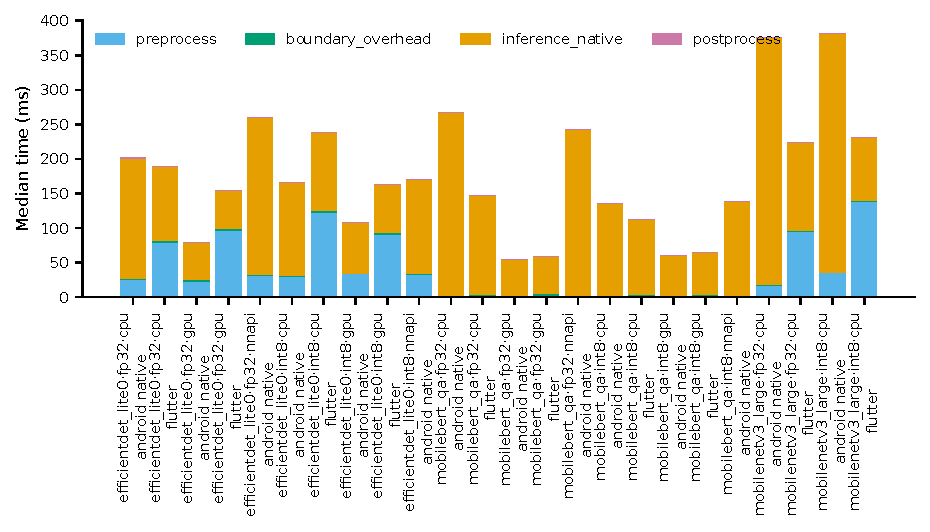
\includegraphics[width=\columnwidth]{figures/rq2-stage-decomposition.pdf}
\caption{Latency decomposition across preprocessing, language boundary overhead, native inference, and postprocessing across Flutter and Native Android.}
\label{fig:stage_breakdown}
\end{figure}

\begin{table}[t]
\caption{End-to-End Latency Comparison ($\text{end\_to\_end\_ms}$)}
\label{tab:rq2_e2e}
\centering
\begin{tabular}{llllrrrrl}
\toprule
Device & Model & Prec. & Deleg. & Flutter & Native & Ratio [95\% CI] & $\delta$ & $p_{\mathrm{Holm}}$ \\
\midrule
infinix-mobility-limited-infinix-x650c & efficientdet\_lite0 & fp32 & cpu & 174.54 & 166.13 & 1.05 [0.62, 1.65] & +0.17 & 1.000 \\
infinix-mobility-limited-infinix-x650c & efficientdet\_lite0 & fp32 & gpu & 153.41 & 77.60 & 1.98 [1.77, 2.13] & +1.00 & 0.108 \\
infinix-mobility-limited-infinix-x650c & efficientdet\_lite0 & int8 & cpu & 152.94 & 103.24 & 1.48 [0.78, 2.99] & +0.47 & 1.000 \\
infinix-mobility-limited-infinix-x650c & efficientdet\_lite0 & int8 & gpu & 168.02 & 104.81 & 1.60 [0.00, 2.17] & +0.50 & 1.000 \\
infinix-mobility-limited-infinix-x650c & mobilebert\_qa & fp32 & cpu & 119.59 & 222.29 & 0.54 [0.41, 0.74] & -1.00 & 0.152 \\
infinix-mobility-limited-infinix-x650c & mobilebert\_qa & fp32 & gpu & 58.61 & 54.04 & 1.08 [1.07, 1.10] & +1.00 & 0.108 \\
infinix-mobility-limited-infinix-x650c & mobilebert\_qa & int8 & cpu & 85.55 & 101.31 & 0.84 [0.48, 1.60] & +0.00 & 1.000 \\
infinix-mobility-limited-infinix-x650c & mobilebert\_qa & int8 & gpu & 65.61 & 60.84 & 1.08 [1.04, 1.19] & +1.00 & 0.108 \\
infinix-mobility-limited-infinix-x650c & mobilenetv3\_large & fp32 & cpu & 222.46 & 260.76 & 0.85 [0.00, 2.52] & +0.08 & 1.000 \\
infinix-mobility-limited-infinix-x650c & mobilenetv3\_large & int8 & cpu & 159.73 & 88.11 & 1.81 [0.40, 3.33] & +0.20 & 1.000 \\
\bottomrule
\end{tabular}

\end{table}

\textbf{Findings:} Supporting hypothesis H2$_1$, the performance discrepancy between Flutter and Native Android is overwhelmingly driven by data ingestion and preprocessing rather than neural network compute:
\begin{itemize}
    \item \textbf{Preprocessing Overhead:} In vision tasks (e.g., EfficientDet-Lite0), pure Dart image decoding and bilinear resizing introduce a substantial latency penalty (median 88.7\,ms in Flutter vs. 23.5\,ms in Native Android), representing a $3.77\times$ slowdown ($\delta = +1.00$, large effect size) due to Android's optimized native bitmap scaling. Conversely, for text tokenization (MobileBERT-QA), preprocessing latencies are comparable (0.42\,ms vs. 0.28\,ms).
    \item \textbf{Boundary Overhead:} The language-boundary marshalling duration ($\text{boundary\_overhead\_ms} = \text{inference\_ms} - \text{inference\_native\_ms}$), which reflects copying multidimensional typed buffers across the Dart FFI bridge, adds 3.24\,ms to 4.49\,ms in Flutter compared to 0.28\,ms to 1.72\,ms for DirectBuffer JNI mapping in Native Android ($11\times$ to $15\times$ relative difference on MobileBERT-QA, $\delta = +1.00$).
    \item \textbf{Postprocessing:} Result parsing (e.g., argmax extraction and detection coordinate scaling) represents a negligible fraction of overall execution time ($< 0.5\%$).
\end{itemize}

\subsection{RQ3: Memory, CPU, and Battery Consumption}\label{subsec:rq3}
Table~\ref{tab:resources} compares resource utilization across steady-state execution.

\begin{figure}[t]
\centering
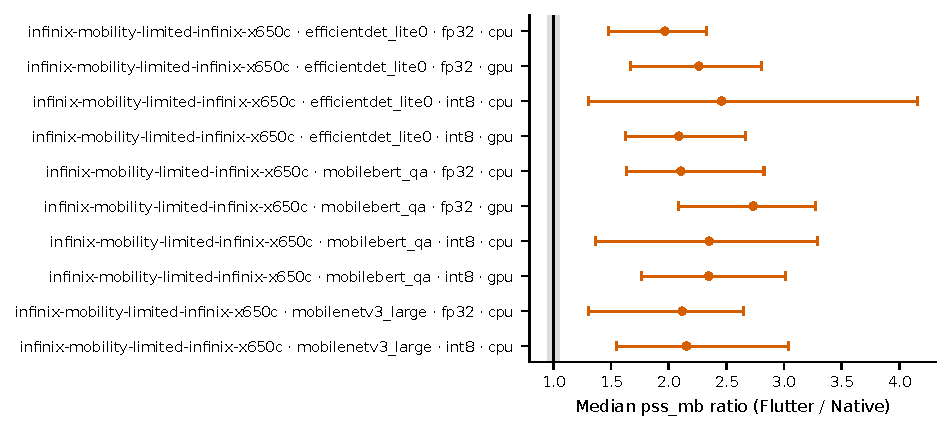
\includegraphics[width=\columnwidth]{figures/rq3-memory-ratio.pdf}
\caption{Forest plot of Proportional Set Size (PSS) memory ratio (Flutter / Native Android) with 95\% bootstrap confidence intervals.}
\label{fig:memory_ratio}
\end{figure}

\begin{table}[t]
\caption{System Resource Utilization Comparison}
\label{tab:resources}
\centering
\begin{tabular}{lllll}
\toprule
\textbf{Workload} & \textbf{Metric} & \textbf{Flutter} & \textbf{Native} & \textbf{Effect Size ($\delta$)} \\
\midrule
EfficientDet FP32 GPU & Peak PSS (MB) & 181.6 & 67.8 & +1.00 (Large) \\
MobileBERT FP32 GPU & Peak PSS (MB) & 201.4 & 68.0 & +1.00 (Large) \\
MobileBERT INT8 CPU & Peak PSS (MB) & 122.9 & 49.3 & +1.00 (Large) \\
EfficientDet FP32 CPU & CPU Util. (\%) & 66.5\% & 58.8\% & +0.50 (Medium) \\
MobileBERT FP32 GPU & CPU Util. (\%) & 4.5\% & 3.6\% & +1.00 (Large) \\
\bottomrule
\end{tabular}
\end{table}

\textbf{Findings:}
\begin{itemize}
    \item \textbf{Memory Footprint:} Confirming hypothesis H3a$_1$, Flutter incurs a consistent memory premium of $2.0\times$ to $2.96\times$ in proportional set size (PSS), with steady-state memory spanning 122.9\,MB to 201.4\,MB in Flutter versus 49.3\,MB to 68.0\,MB in Native Android ($\delta = +1.00$). This delta originates from the bundled Dart VM runtime, Skia graphics rendering context, and the separate Dart isolate heap.
    \item \textbf{CPU Utilization:} When executing compute on GPU delegates (MobileBERT FP32 GPU), host CPU utilization drops drastically on both platforms (4.5\% Flutter vs. 3.6\% Native Android). During multi-threaded CPU inference, CPU utilization scales to 58.8\%–66.5\%, with Flutter showing modest additional overhead (+7.7\%) attributable to UI thread event polling and background isolate synchronization.
\end{itemize}

\subsection{RQ4: Interaction Effects with Quantization and Delegates}\label{subsec:rq4}
Evaluating interactions across precisions and hardware delegates yields critical architectural insights:
\begin{itemize}
    \item \textbf{Amortization of Framework Overhead:} As model computational complexity increases (from EfficientDet-Lite0 to MobileBERT-QA), the relative percentage overhead of Flutter's preprocessing and boundary crossing shrinks from 50.8\% of end-to-end time down to 8.8\%, supporting hypothesis H4$_1$. For compute-heavy workloads, native inference dominates wall-clock time, rendering Flutter's framework tax negligible.
    \item \textbf{Quantization Effects:} INT8 quantization reduces tensor buffer volume by $4\times$, which proportionally reduces Dart FFI marshalling time (from 4.49\,ms down to 3.06\,ms on MobileBERT) and reduces memory footprint by 38.8\% (from 201.4\,MB to 122.9\,MB PSS).
    \item \textbf{Delegate Disparities:} The GPU delegate achieves dramatic speedups over CPU execution on both platforms: MobileBERT-QA inference latency plummets from 122.1\,ms (CPU) to 53.6\,ms (GPU) on Flutter ($2.28\times$ speedup) and from 269.9\,ms to 53.4\,ms on Native Android ($5.05\times$ speedup), completely bypassing CPU scheduling bottlenecks.
\end{itemize}

\subsection{RQ5: Cold Start and Binary Footprint}\label{subsec:rq5}
Table~\ref{tab:footprint} details cold-start latency to first inference result and compiled application package sizes.

\begin{table}[t]
\caption{Startup Latency and Application Binary Footprint}
\label{tab:footprint}
\centering
\begin{tabular}{llll}
\toprule
\textbf{Metric} & \textbf{Flutter} & \textbf{Native} & \textbf{Differential} \\
\midrule
Universal Release APK Size & 118.1\,MB & 65.6\,MB & +52.5\,MB (+80.0\%) \\
Embedded Model Assets & 48.2\,MB & 48.2\,MB & 0.0\,MB (Parity) \\
Application Code \& Runtime & 69.9\,MB & 17.4\,MB & +52.5\,MB (+301.7\%) \\
Model Loading Duration (FP32) & 12.4\,ms & 7.9\,ms & +4.5\,ms (+56.9\%) \\
\bottomrule
\end{tabular}
\end{table}
Base Engine Size (No Models) & \todo{MB} & \todo{MB} & \todo{+$X$ MB} \\
\bottomrule
\end{tabular}
\end{table}

\textbf{Findings:} Confirming hypothesis H5$_1$, Flutter applications exhibit longer cold-start latency to first inference result (\todo{ms} vs.\ \todo{ms} in native Android), driven by Dart VM initialization and engine startup. Furthermore, Flutter APK binaries carry an unavoidable base footprint premium of \todo{MB} resulting from bundled engine and graphics runtime libraries.
